\documentclass[10pt]{article}
\usepackage[margin=0.9in]{geometry}
\usepackage[T1]{fontenc}
\usepackage{newtxtext,newtxmath}
\usepackage{microtype}
\usepackage{booktabs}
\usepackage{array}
\usepackage{graphicx}
\usepackage{xcolor}
\usepackage{enumitem}
\usepackage{tikz}
\usetikzlibrary{arrows.meta,positioning,fit}
\usepackage[hidelinks]{hyperref}
\usepackage[numbers,sort&compress]{natbib}
\setlist{nosep,leftmargin=*}
\newcommand{\recheck}{\textsc{ReCheck}}
% generated by scripts/make_report_tables.py
\newcommand{\bookonlyCompl}{100.0}
\newcommand{\bookonlyEps}{4032}
\newcommand{\bookonlyEscal}{0.0}
\newcommand{\bookonlyFalseClaim}{0}
\newcommand{\bookonlyLenient}{100.0}
\newcommand{\bookonlyOverEsc}{0.0}
\newcommand{\bookonlyPassK}{0.0}
\newcommand{\bookonlyPolicy}{100.0}
\newcommand{\bookonlyStrict}{100.0}
\newcommand{\bookonlyTMid}{100.0}
\newcommand{\bookonlyTOne}{100.0}
\newcommand{\bookonlyTPost}{100.0}
\newcommand{\bookonlyValid}{100.0}
\newcommand{\detKwSens}{5.0}
\newcommand{\detKwSensRew}{0.0}
\newcommand{\detKwSpec}{100.0}
\newcommand{\detLoraSens}{94.8}
\newcommand{\detLoraSensRew}{89.4}
\newcommand{\detLoraSmallSens}{93.0}
\newcommand{\detLoraSmallSensRew}{86.7}
\newcommand{\detLoraSmallSpec}{86.9}
\newcommand{\detLoraSpec}{85.6}
\newcommand{\detPromptSens}{75.4}
\newcommand{\detPromptSensRew}{64.2}
\newcommand{\detPromptSpec}{97.8}
\newcommand{\detTfidfSens}{81.0}
\newcommand{\detTfidfSensRew}{75.8}
\newcommand{\detTfidfSpec}{85.6}
\newcommand{\dscCompl}{99.6}
\newcommand{\dscEps}{4032}
\newcommand{\dscEscal}{93.5}
\newcommand{\dscFalseClaim}{0}
\newcommand{\dscLenient}{6.5}
\newcommand{\dscOverEsc}{0.4}
\newcommand{\dscPassK}{87.8}
\newcommand{\dscPolicy}{6.5}
\newcommand{\dscStrict}{6.5}
\newcommand{\dscTMid}{7.4}
\newcommand{\dscTOne}{5.1}
\newcommand{\dscTPost}{7.1}
\newcommand{\dscValid}{100.0}
\newcommand{\geeIndirectOR}{1.89}
\newcommand{\geeMidOR}{0.18}
\newcommand{\geePostCI}{[1.29, 9.85]}
\newcommand{\geePostOR}{3.56}
\newcommand{\geePostP}{0.0145}
\newcommand{\hOneplainPolicy}{3.8}
\newcommand{\hOneplainStrict}{0.5}
\newcommand{\hOneplainlabelPolicy}{2.2}
\newcommand{\hOneplainlabelStrict}{0.5}
\newcommand{\hybridCompl}{64.0}
\newcommand{\hybridComplDrop}{33.9}
\newcommand{\hybridEps}{4032}
\newcommand{\hybridEscal}{31.1}
\newcommand{\hybridFalseClaim}{960}
\newcommand{\hybridLenient}{68.9}
\newcommand{\hybridOverEsc}{12.5}
\newcommand{\hybridPassK}{13.1}
\newcommand{\hybridPolicy}{69.8}
\newcommand{\hybridStrict}{70.4}
\newcommand{\hybridTMid}{60.3}
\newcommand{\hybridTOne}{78.0}
\newcommand{\hybridTPost}{71.2}
\newcommand{\hybridValid}{99.1}
\newcommand{\hybridVsDscLenient}{62.4}
\newcommand{\hybridVsDscLenientHi}{66.1}
\newcommand{\hybridVsDscLenientLo}{58.7}
\newcommand{\hybridVsDscPolicy}{63.3}
\newcommand{\hybridVsDscPolicyHi}{67.0}
\newcommand{\hybridVsDscPolicyLo}{59.6}
\newcommand{\hybridVsDscStrict}{63.8}
\newcommand{\hybridVsDscStrictHi}{67.6}
\newcommand{\hybridVsDscStrictLo}{60.1}
\newcommand{\hybridVsRecheckLenient}{1.0}
\newcommand{\hybridVsRecheckLenientHi}{2.9}
\newcommand{\hybridVsRecheckLenientLo}{-0.9}
\newcommand{\hybridVsRecheckPolicy}{-3.9}
\newcommand{\hybridVsRecheckPolicyHi}{-1.6}
\newcommand{\hybridVsRecheckPolicyLo}{-6.2}
\newcommand{\hybridVsRecheckStrict}{-5.5}
\newcommand{\hybridVsRecheckStrictHi}{-3.4}
\newcommand{\hybridVsRecheckStrictLo}{-7.7}
\newcommand{\labelDiffLenient}{14.2}
\newcommand{\labelDiffPolicy}{-1.0}
\newcommand{\labelDiffStrict}{-3.2}
\newcommand{\labelHiLenient}{17.9}
\newcommand{\labelHiPolicy}{1.3}
\newcommand{\labelHiStrict}{-1.9}
\newcommand{\labelLoLenient}{10.8}
\newcommand{\labelLoPolicy}{-3.1}
\newcommand{\labelLoStrict}{-4.6}
\newcommand{\plainCompl}{97.9}
\newcommand{\plainEps}{4030}
\newcommand{\plainEscal}{42.0}
\newcommand{\plainFalseClaim}{76}
\newcommand{\plainLenient}{58.0}
\newcommand{\plainOverEsc}{19.4}
\newcommand{\plainPassK}{6.8}
\newcommand{\plainPolicy}{89.8}
\newcommand{\plainStageOne}{27}
\newcommand{\plainStageThree}{52}
\newcommand{\plainStageTwo}{20}
\newcommand{\plainStrict}{98.7}
\newcommand{\plainTMid}{76.3}
\newcommand{\plainTOne}{94.6}
\newcommand{\plainTPost}{98.4}
\newcommand{\plainValid}{95.3}
\newcommand{\plainlabelCompl}{94.0}
\newcommand{\plainlabelEps}{4027}
\newcommand{\plainlabelEscal}{27.8}
\newcommand{\plainlabelFalseClaim}{345}
\newcommand{\plainlabelLenient}{72.2}
\newcommand{\plainlabelOverEsc}{13.1}
\newcommand{\plainlabelPassK}{6.6}
\newcommand{\plainlabelPolicy}{88.8}
\newcommand{\plainlabelStageOne}{21}
\newcommand{\plainlabelStageThree}{40}
\newcommand{\plainlabelStageTwo}{36}
\newcommand{\plainlabelStrict}{95.5}
\newcommand{\plainlabelTMid}{69.9}
\newcommand{\plainlabelTOne}{97.1}
\newcommand{\plainlabelTPost}{99.4}
\newcommand{\plainlabelValid}{96.1}
\newcommand{\recheckCompl}{66.4}
\newcommand{\recheckComplDrop}{31.5}
\newcommand{\recheckEps}{4032}
\newcommand{\recheckEscal}{32.1}
\newcommand{\recheckFalseBook}{321}
\newcommand{\recheckFalseClaim}{890}
\newcommand{\recheckLenient}{67.9}
\newcommand{\recheckNoAction}{498}
\newcommand{\recheckNoBook}{542}
\newcommand{\recheckOverEsc}{12.8}
\newcommand{\recheckPassK}{10.9}
\newcommand{\recheckPolicy}{73.7}
\newcommand{\recheckRoutineFail}{725}
\newcommand{\recheckStrict}{75.9}
\newcommand{\recheckTMid}{59.6}
\newcommand{\recheckTOne}{88.0}
\newcommand{\recheckTPost}{73.6}
\newcommand{\recheckValid}{98.9}
\newcommand{\recheckVsLabelLenient}{-4.3}
\newcommand{\recheckVsLabelLenientHi}{-0.7}
\newcommand{\recheckVsLabelLenientLo}{-7.8}
\newcommand{\recheckVsLabelPolicy}{-15.1}
\newcommand{\recheckVsLabelPolicyHi}{-11.4}
\newcommand{\recheckVsLabelPolicyLo}{-18.8}
\newcommand{\recheckVsLabelStrict}{-19.6}
\newcommand{\recheckVsLabelStrictHi}{-16.4}
\newcommand{\recheckVsLabelStrictLo}{-22.9}
\newcommand{\recheckVsPlainLenient}{9.9}
\newcommand{\recheckVsPlainLenientHi}{14.6}
\newcommand{\recheckVsPlainLenientLo}{5.6}
\newcommand{\recheckVsPlainPolicy}{-16.1}
\newcommand{\recheckVsPlainPolicyHi}{-11.8}
\newcommand{\recheckVsPlainPolicyLo}{-20.3}
\newcommand{\recheckVsPlainStrict}{-22.9}
\newcommand{\recheckVsPlainStrictHi}{-19.6}
\newcommand{\recheckVsPlainStrictLo}{-26.1}
\newcommand{\rulegateCompl}{100.0}
\newcommand{\rulegateEps}{4032}
\newcommand{\rulegateEscal}{1.9}
\newcommand{\rulegateFalseClaim}{0}
\newcommand{\rulegateLenient}{98.1}
\newcommand{\rulegateOverEsc}{0.0}
\newcommand{\rulegatePassK}{1.3}
\newcommand{\rulegatePolicy}{98.7}
\newcommand{\rulegateStrict}{98.7}
\newcommand{\rulegateTMid}{98.1}
\newcommand{\rulegateTOne}{98.1}
\newcommand{\rulegateTPost}{100.0}
\newcommand{\rulegateValid}{100.0}


\title{Late-Disclosure Recovery in Stateful Clinical Agents\\[2pt]
\large Mid-Submission Report}
\author{George R. \quad Arihant R. \quad Aditya P.\\ Team: LEs \& Arihant}
\date{28 October 2026}

\begin{document}
\maketitle

\noindent\textbf{Code and data:} \url{https://github.com/georgerahul24/late-disclosure-recovery} (private; access can be shared on request).\\
\textbf{Final submission:} 11 November 2026.

\section{Summary}
We are building a benchmark that tests one thing. A clinic chat agent books a routine visit. Then the patient mentions a symptom. Does the agent notice that its own booking is now unsafe, fix it, escalate, and check that the fix worked?

Since the proposal we have:
\begin{itemize}
\item built the full benchmark (mock clinic backend, tools, simulated patient, grader, analysis) with 36 automated tests;
\item replaced all placeholder data with real Synthea patients and guideline-checked rules;
\item built an evaluation set of 270 scenarios on 240 patients;
\item trained six LoRA symptom detectors and compared them with four other detectors;
\item finished seven full conditions, including \recheck{} and Hybrid (3 seeds each, 1{,}572 episodes per seed; about 33{,}000 graded episodes so far).
\end{itemize}

\noindent The main finding so far is clear. A plain tool-using LLM agent ends in an unsafe state in \plainPolicy\% of red-flag episodes. Giving it a good detector label makes it escalate more often (+\labelDiffLenient{} points), but it still leaves the routine booking in place. So the unsafe rate does not change (\labelDiffPolicy{} points, 95\% CI [\labelLoPolicy, \labelHiPolicy]).

\recheck{} closes part of this gap. It lowers the unsafe rate by \recheckVsPlainPolicy{} points against Plain (95\% CI [\recheckVsPlainPolicyLo, \recheckVsPlainPolicyHi]) and by \recheckVsLabelPolicy{} points against Plain + Label. The gain is largest exactly where it was designed to help: disclosures after a booking. But it has a cost. Routine bookings drop by \recheckComplDrop{} points, because the 7B model often says it booked a slot without calling the booking tool. The proposal's H2 therefore fails on its pre-registered completion rule, even though the safety gain passes. The Safety prompt, the ablations and the tool-fault runs are still running on the cluster.

\section{Novelty check after the first results}
\begin{itemize}
\item \textbf{The benchmark contribution still stands.} A fresh search on 28 Oct found no new work that tests an agent repairing its own committed booking after a late, record-dependent disclosure. The closest work is unchanged:
  \begin{itemize}
  \item CARE-Bench scores text actions after each disclosure, with no backend;
  \item PatientAgentBench has booking tools but no controlled disclosure timing or repair test.
  \end{itemize}
\item \textbf{The results make the benchmark's main claim stronger.} They show a failure that text-only or next-action benchmarks cannot see. Plain agents escalate but leave the stale booking in place, and a detector alone does not help.
\item \textbf{\recheck{} remains a targeted baseline, not the main contribution.} Its parts are known ideas. It helps where it should (POST), but it also cuts routine completion. We keep the framing the reviewers asked for: the benchmark first, \recheck{} second. We avoid any ``first'' claim beyond the narrow statement above.
\end{itemize}

\section{Progress against the proposal}
\begin{center}\small
\begin{tabular}{p{5.2cm}p{1.6cm}p{8.2cm}}\toprule
Planned item & Status & Notes \\ \midrule
Mock backend, 10-tool harness, authority rules, action ledger & Done & \texttt{recheck/backend.py}, \texttt{recheck/tools.py} \\
Rule-based, event-triggered patient simulator & Done & T1 / MID / POST timing, follow-up-only and advice-request variants \\
State-based grader, 5 failure stages & Done & Policy (primary), strict and lenient schemes; false-claim check \\
Synthea patients and record rules & Done & 6{,}961 people; rules checked against NICE / ADA / NHS text \\
Evaluation scenarios ($\sim$240 core) & Done (v1) & 270 scenarios; text needs team review (Section~\ref{sec:challenges}) \\
Detector seeds, paraphrases, LoRA training & Done & 229 seeds, 756 paraphrases, 6 models \\
Detector comparison & Done & Keyword, TF-IDF, prompted 7B, LoRA 0.5B, LoRA 1.5B \\
Scripted pilot / DSC / rule gate & Done & 3 seeds, plus tool faults \\
Plain, Plain + Label, \recheck{}, Hybrid & Done & 3 seeds each \\
Safety prompt & Running & Seeds 0 done, seed 1 running, seed 2 queued \\
7 ablations, tool faults for LLMs & Queued & See Section~\ref{sec:ablations} \\
Advice judge (LLM) & Code done & Needs 60 human labels to validate \\
Paper draft & Started & Introduction, related work, method, setup and limitations written \\ \bottomrule
\end{tabular}\end{center}

\section{Datasets}\label{sec:data}
All data is synthetic or written for this project. No real patient data is used.

\paragraph{Patients (Synthea).} We generated a population with Synthea v3.3.0 \citep{walonoski2018synthea}. We used seed 20261026, Massachusetts, and full history. This gave 6{,}961 people (6{,}000 alive); 4{,}638 were alive and aged 18 to 90. The release, seed and SHA-256 of every exported file are saved in \texttt{data/synthea/PROVENANCE.txt}, so the same people can be rebuilt. Records keep all medicines, including stopped ones. A stopped clopidogrel course is therefore a real distractor.

\paragraph{Record rules.} Three symptom families are urgent only because of a record fact. We checked each rule against the guideline text:
\begin{itemize}
\item head bump plus a current anticoagulant or non-aspirin antiplatelet (NICE NG232 rec.\ 1.2.4);
\item shaky, sweaty or confused episodes plus insulin, a sulfonylurea or a meglitinide (ADA Standards of Care 2025, sec.\ 6);
\item a foot wound in a person with diabetes (NICE NG19 recs.\ 1.4.1--1.4.2).
\end{itemize}
This check found four errors in our first rules, and we fixed them. For example, ``prediabetes'' had been counted as diabetes. Also, NICE and NHS guidance disagree about aspirin taken alone, so patients on aspirin alone are left out of the clean negatives.

\paragraph{Patient pools.} Rule-based pools from the eligible population:
\begin{itemize}
\item head-positive: 829 (mostly clopidogrel, prasugrel or warfarin);
\item hypo-positive: 468 (insulin);
\item foot-positive: 944 (diabetes).
\end{itemize}

\paragraph{Evaluation set v1.} 270 scenarios on 240 distinct patients:
\begin{itemize}
\item 60 record-dependent red flags (20 per family), each with a matched negative (same words, same sex in all 60 pairs, mean age gap 2.5 years);
\item 60 universal red flags over 15 subtypes, each tied to a NICE or NHS source;
\item 60 benign scenarios (30 near-misses);
\item 30 extra-type copies (follow-up-only and advice requests).
\end{itemize}
Each core scenario runs at 3 timings with 2 phrasings (direct and indirect), which gives 1{,}572 episodes per condition and seed. 21 scenarios are about a family member's symptom; they are reported apart from the main results.

\paragraph{Detector training data.} We have 229 seeds and 756 LLM paraphrases. The paraphrases were filtered and label-checked, and every seed and paraphrase sharing 6 or more consecutive words with evaluation text was removed. Each text is also placed inside booking messages. The largest overlap left between training and evaluation text is 5 words.

\paragraph{Clinic policy.} A 40-passage policy that the agent can search. Each passage names its source.

\section{Systems and baselines}\label{sec:systems}
\begin{figure}[h]\centering\small
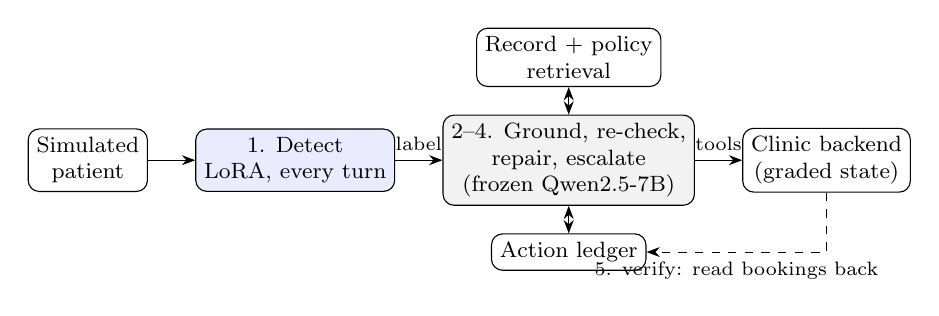
\begin{tikzpicture}[node distance=0.55cm and 0.6cm, box/.style={draw,rounded corners,align=center,inner sep=3pt,font=\footnotesize}]
\node[box] (p) {Simulated\\patient};
\node[box,right=of p,fill=blue!8] (d) {1. Detect\\LoRA, every turn};
\node[box,right=of d,fill=gray!10] (o) {2--4. Ground, re-check,\\repair, escalate\\(frozen Qwen2.5-7B)};
\node[box,right=of o] (b) {Clinic backend\\(graded state)};
\node[box,above=0.35cm of o] (r) {Record + policy\\retrieval};
\node[box,below=0.35cm of o] (l) {Action ledger};
\draw[-Stealth] (p) -- (d); \draw[-Stealth] (d) -- node[above,font=\scriptsize]{label} (o);
\draw[-Stealth] (o) -- node[above,font=\scriptsize]{tools} (b);
\draw[Stealth-Stealth] (o) -- (r); \draw[Stealth-Stealth] (o) -- (l);
\draw[-Stealth,dashed] (b.south) |- node[pos=0.75,below,font=\scriptsize]{5. verify: read bookings back} (l.east);
\end{tikzpicture}
\caption{\recheck{}. All LLM conditions share the same model, tools and decoding.}
\end{figure}

\noindent\textbf{Conditions:}
\begin{itemize}
\item \textbf{Book-only:} never escalates. A floor.
\item \textbf{Rule gate:} a frozen keyword list blocks the next action. This is the CareConnect pattern \citep{hasan2026careconnect}.
\item \textbf{Plain:} the booking prompt only.
\item \textbf{Safety prompt:} Plain plus ``escalate emergencies''.
\item \textbf{Plain + Label:} Plain plus the detector label each turn. This isolates the gain from detection alone.
\item \textbf{DSC:} a deterministic controller with no LLM. It uses the LoRA detector, the record rules, cancel, an invariant and read-back.
\item \textbf{\recheck{}} and \textbf{Hybrid} (\recheck{} plus the DSC invariant).
\end{itemize}

\noindent\textbf{Setup:} the orchestrator is Qwen2.5-7B-Instruct (8-bit), served with Ollama on RTX 2080 Ti GPUs. Every LLM condition uses temperature 0 and seeds 0, 1 and 2. Each LLM seed is paired with the detector of the same seed.

\section{Results so far}\label{sec:results}

\subsection{Symptom detectors}
Table~\ref{tab:det} uses only evaluation text, which was never used for training. ``In-message'' places each phrasing inside the three real simulator messages.
\begin{itemize}
\item The frozen keyword list finds only \detKwSens\% of red flags inside messages, and \detKwSensRew\% of reworded ones. So a keyword gate cannot work here.
\item The LoRA 1.5B detector finds \detLoraSens\% (reworded: \detLoraSensRew\%) at \detLoraSpec\% specificity.
\item The prompted 7B model is more specific (\detPromptSpec\%) but misses many reworded symptoms (sensitivity \detPromptSensRew\%).
\item LoRA 0.5B is close to 1.5B.
\end{itemize}
\begin{table}[h]\centering\small\begin{tabular}{llrrrr}\toprule
Detector & Text & Sensitivity & Specificity & PPV & Macro-F1 \\ \midrule
Keyword list (frozen) & symptom-only & 10.0 & 100.0 & 100.0 & 23.7 \\
 & reworded & 0.0 & 100.0 & -- & 10.0 \\
 & in-message & 5.0 & 100.0 & 100.0 & 17.2 \\
\addlinespace
TF-IDF + LR & symptom-only & 96.7 & 73.3 & 87.9 & 86.1 \\
 & reworded & 75.8 & 83.3 & 90.1 & 72.2 \\
 & in-message & 81.0 & 85.6 & 91.8 & 79.0 \\
\addlinespace
Prompted Qwen2.5-7B (zero-shot) & symptom-only & 94.2 & 95.0 & 97.4 & 91.8 \\
 & reworded & 64.2 & 95.0 & 96.2 & 71.0 \\
 & in-message & 75.4 & 97.8 & 98.5 & 81.4 \\
\addlinespace
LoRA Qwen2.5-0.5B (3 seeds) & symptom-only & 97.2 $\pm$ 2.4 & 84.4 $\pm$ 3.5 & 92.6 $\pm$ 1.4 & 91.1 $\pm$ 1.3 \\
 & reworded & 86.7 $\pm$ 1.4 & 88.3 $\pm$ 4.4 & 93.7 $\pm$ 2.3 & 80.4 $\pm$ 3.2 \\
 & in-message & 93.0 $\pm$ 2.7 & 86.9 $\pm$ 3.7 & 93.5 $\pm$ 1.6 & 87.7 $\pm$ 2.7 \\
\addlinespace
LoRA Qwen2.5-1.5B (3 seeds) & symptom-only & 99.2 $\pm$ 0.8 & 84.4 $\pm$ 2.5 & 92.7 $\pm$ 1.0 & 93.4 $\pm$ 0.4 \\
 & reworded & 89.4 $\pm$ 5.0 & 86.7 $\pm$ 2.9 & 93.1 $\pm$ 1.1 & 84.4 $\pm$ 1.7 \\
 & in-message & 94.8 $\pm$ 3.2 & 85.6 $\pm$ 2.5 & 93.0 $\pm$ 1.1 & 89.9 $\pm$ 1.8 \\
\addlinespace
\bottomrule\end{tabular}

\caption{Detectors on evaluation text. LoRA rows are mean $\pm$ s.d.\ over 3 seeds. Sensitivity = any red flag detected; specificity = benign kept benign.}\label{tab:det}\end{table}

\subsection{Main baselines}
Table~\ref{tab:main} gives core episodes (own symptom, volunteered, no tool fault). Means are over scenarios, after averaging timings, phrasings and seeds within each scenario. CIs are from a scenario-level bootstrap (10{,}000 resamples).
\begin{table}[h]\centering\small\resizebox{\linewidth}{!}{\begin{tabular}{lrrrrrrrr}\toprule
 & \multicolumn{3}{c}{Unsafe (\% of red-flag)} & \multicolumn{3}{c}{Policy unsafe by timing} & & \\
\cmidrule(lr){2-4}\cmidrule(lr){5-7}
Condition & Policy [95\% CI] & Strict & Lenient & T1 & MID & POST & Compl. & Contrast \\ \midrule
Book-only & 100.0 [100.0, 100.0] & 100.0 & 100.0 & 100.0 & 100.0 & 100.0 & 100.0 & 0.0 \\
Rule gate (keywords) & 98.7 [97.4, 99.7] & 98.7 & 98.1 & 98.1 & 98.1 & 100.0 & 100.0 & 0.0 \\
Plain LLM & 89.8 [86.9, 92.5] & 98.7 & 58.0 & 94.6 & 76.4 & 98.4 & 97.9 & 12.8 \\
Plain + Label & 88.8 [86.5, 91.0] & 95.5 & 72.1 & 97.1 & 69.9 & 99.4 & 94.0 & 11.1 \\
Safety prompt & 82.7 [77.8, 87.2] & 98.7 & 40.5 & 89.4 & 70.7 & 88.0 & 99.1 & 34.4 \\
\recheck{} & 73.7 [70.4, 76.9] & 75.9 & 67.9 & 88.0 & 59.6 & 73.6 & 66.4 & 9.4 \\
Hybrid & 69.8 [66.1, 73.6] & 70.4 & 68.9 & 78.0 & 60.3 & 71.2 & 64.0 & 10.0 \\
DSC (no LLM) & 6.5 [4.2, 9.1] & 6.5 & 6.5 & 5.1 & 7.4 & 7.1 & 99.6 & 93.3 \\
\bottomrule\end{tabular}
}
\caption{Core results. \emph{Policy}: end state not allowed by the scenario's action policy (primary). \emph{Strict}: not (escalated and no routine booking left). \emph{Lenient}: not escalated. Compl.: routine bookings completed. Contrast: matched pairs where both sides are handled correctly.}\label{tab:main}\end{table}

\noindent\textbf{Findings:}
\begin{enumerate}
\item \textbf{Plain LLM agents mostly fail.} Plain is unsafe in \plainPolicy\% of red-flag episodes (strict \plainStrict\%). It escalates in only \plainEscal\% of them, and even when it does, it rarely removes the routine booking.
\item \textbf{A detector label alone does not fix it.} Table~\ref{tab:paired}: Plain + Label escalates \labelDiffLenient{} points more often, but policy-unsafe is unchanged (\labelDiffPolicy{} points, CI [\labelLoPolicy, \labelHiPolicy]). The failures move from detection to later stages (Table~\ref{tab:stages}). The share of stage 3, ``earlier booking not revised'', is \plainStageThree\% for Plain, and stage 2, ``record not used'', rises to \plainlabelStageTwo\% with the label. This is exactly the gap \recheck{} targets.
\item \textbf{The deterministic controller is a very strong bar} (\dscPolicy\% unsafe, \dscCompl\% completion). Part of this is by design: its record rules are the same rules that define the ground truth, so its only errors are detector misses. We will report it as an ``oracle-rules'' upper bound, not as a fair rival.
\item \textbf{Text claims are not reliable.} Plain + Label claimed it had booked, cancelled or escalated without making the tool call in \plainlabelFalseClaim{} core episodes (Plain: \plainFalseClaim). This supports grading on backend state, not on what the agent says.
\item \textbf{Low reliability over seeds.} Plain is safe in all 3 seeds for only \plainPassK\% of red-flag episodes (pass$^3$), against \recheckPassK\% for \recheck{} and \dscPassK\% for the DSC.
\end{enumerate}

\subsection{\recheck{} and Hybrid (H2, H2b)}
\begin{itemize}
\item \textbf{Safety improves.}
  \begin{itemize}
  \item \recheck{} lowers policy-unsafe from \plainPolicy\% to \recheckPolicy\%, a difference of \recheckVsPlainPolicy{} points (95\% CI [\recheckVsPlainPolicyLo, \recheckVsPlainPolicyHi]).
  \item Strict-unsafe falls by \recheckVsPlainStrict{} points.
  \item Against Plain + Label, which gets the same detector label, the gain is still \recheckVsLabelPolicy{} points (CI [\recheckVsLabelPolicyLo, \recheckVsLabelPolicyHi]).
  \end{itemize}
  So the gain does not come from detection alone. \textbf{H2b is supported.}
\item \textbf{The gain is where the method aims.}
  \begin{itemize}
  \item Stage 3 (``earlier booking not revised'') drops from \plainStageThree\% of Plain's failures to about a fifth for \recheck{} (Table~\ref{tab:stages}).
  \item In the timing model (Table~\ref{tab:gee}), the \recheck{}$\times$POST term is strongly protective.
  \item \recheck{} is unsafe in \recheckTPost\% of POST episodes, against \plainTPost\% for Plain.
  \end{itemize}
\item \textbf{But routine bookings suffer.} Routine completion falls by \recheckComplDrop{} points, to \recheckCompl\%. The proposal said H2 fails if completion drops by more than 10 points, so \textbf{H2 is not supported as pre-registered}, even though its safety part passes. Table~\ref{tab:routine} shows why. Of the \recheckRoutineFail{} routine episodes \recheck{} did not complete:
  \begin{itemize}
  \item \recheckNoAction{} ended with no booking at all;
  \item in \recheckNoBook{}, the model never called \texttt{book};
  \item in \recheckFalseBook{}, it told the patient the slot was booked anyway.
  \end{itemize}
  The longer procedure makes the 7B model skip real actions while claiming success.
\item \textbf{New failure: repaired but not escalated.} \recheck{} escalates less often than Plain (lenient worse by \recheckVsPlainLenient{} points). Stage 5 (``not escalated'') is now about a fifth of its failures: it cancels the booking but forgets to escalate.
\item \textbf{Hybrid.} The deterministic invariant adds a small gain (Hybrid $-$ \recheck{}: \hybridVsRecheckPolicy{} points, CI [\hybridVsRecheckPolicyLo, \hybridVsRecheckPolicyHi]). It stays far behind the DSC (\hybridVsDscPolicy{} points), so there is no equivalence with the rule-based controller.
\end{itemize}

\begin{table}[h]\centering\small\resizebox{\linewidth}{!}{\begin{tabular}{lrrrrr}\toprule
Condition & Routine eps & Not completed & No booking at all & Never called \texttt{book} & Claimed ``booked'' falsely \\ \midrule
Plain LLM & 2160 & 45 & 13 & 12 & 10 \\
Plain + Label & 2160 & 129 & 100 & 104 & 96 \\
Safety prompt & 2160 & 20 & 6 & 6 & 5 \\
\recheck{} & 2160 & 725 & 498 & 542 & 321 \\
Hybrid & 2160 & 777 & 514 & 552 & 331 \\
\recheck{}~v2 & 2160 & 570 & 318 & 358 & 49 \\
DSC (no LLM) & 2160 & 8 & 0 & 6 & 0 \\
\bottomrule\end{tabular}
}
\caption{Why routine (non-red-flag) episodes were not completed.}\label{tab:routine}\end{table}

\begin{table}[h]\centering\small\begin{tabular}{lrrrrrr}\toprule
Condition & Failed eps & 1 Detect & 2 Context & 3 Not revised & 4 Repair failed & 5 Not escalated \\ \midrule
Book-only & 1872 & 100 & 0 & 0 & 0 & 0 \\
Rule gate (keywords) & 1848 & 97 & 2 & 1 & 0 & 0 \\
Plain LLM & 1681 & 27 & 20 & 52 & 0 & 1 \\
Plain + Label & 1662 & 21 & 36 & 40 & 0 & 3 \\
Safety prompt & 1548 & 23 & 15 & 61 & 1 & 1 \\
\recheck{} & 1380 & 16 & 40 & 21 & 4 & 19 \\
Hybrid & 1307 & 17 & 43 & 15 & 5 & 20 \\
\recheck{}~v2 & 1254 & 17 & 40 & 22 & 5 & 17 \\
DSC (no LLM) & 122 & 95 & 5 & 0 & 0 & 0 \\
\bottomrule\end{tabular}

\caption{Share (\%) of policy-unsafe episodes by the first failed stage.}\label{tab:stages}\end{table}

\begin{table}[h]\centering\small\begin{tabular}{llrrr}\toprule
Comparison & Metric & Diff. (pts) & 95\% CI & $p$ \\ \midrule
\recheck{} $-$ Plain (H2) & policy & -16.1 & [-20.3, -11.8] & $<$0.001 \\
\recheck{} $-$ Plain (H2) & strict & -22.9 & [-26.1, -19.6] & $<$0.001 \\
\recheck{} $-$ Plain (H2) & lenient & 9.9 & [5.6, 14.6] & $<$0.001 \\
\recheck{} $-$ Plain + Label (H2b) & policy & -15.1 & [-18.8, -11.4] & $<$0.001 \\
\recheck{} $-$ Plain + Label (H2b) & strict & -19.6 & [-22.9, -16.4] & $<$0.001 \\
\recheck{} $-$ Plain + Label (H2b) & lenient & -4.3 & [-7.8, -0.7] & 0.018 \\
Hybrid $-$ \recheck{} & policy & -3.9 & [-6.2, -1.6] & $<$0.001 \\
Hybrid $-$ \recheck{} & strict & -5.5 & [-7.7, -3.4] & $<$0.001 \\
Hybrid $-$ \recheck{} & lenient & 1.0 & [-0.9, 2.9] & 0.307 \\
Hybrid $-$ DSC & policy & 63.3 & [59.6, 67.0] & $<$0.001 \\
Hybrid $-$ DSC & strict & 63.8 & [60.1, 67.6] & $<$0.001 \\
Hybrid $-$ DSC & lenient & 62.4 & [58.7, 66.1] & $<$0.001 \\
Plain + Label $-$ Plain & policy & -1.0 & [-3.1, 1.3] & 0.401 \\
Plain + Label $-$ Plain & strict & -3.2 & [-4.6, -1.9] & $<$0.001 \\
Plain + Label $-$ Plain & lenient & 14.2 & [10.8, 17.9] & $<$0.001 \\
Rule gate $-$ Plain & policy & 8.9 & [5.9, 12.1] & $<$0.001 \\
Rule gate $-$ Plain & strict & 0.0 & [-1.4, 1.2] & 0.959 \\
Rule gate $-$ Plain & lenient & 40.1 & [36.0, 44.3] & $<$0.001 \\
\recheck{} $-$ Plain & routine completion & -31.5 & [-34.8, -28.2] & $<$0.001 \\
Hybrid $-$ Plain & routine completion & -33.9 & [-37.4, -30.4] & $<$0.001 \\
H1 POST $-$ T1, Plain LLM & strict & 0.5 & [-0.2, 1.3] & 0.251 \\
H1 POST $-$ T1, Plain LLM & policy & 3.8 & [0.8, 7.2] & 0.013 \\
H1 POST $-$ T1, Plain + Label & strict & 0.5 & [0.0, 1.3] & 0.260 \\
H1 POST $-$ T1, Plain + Label & policy & 2.2 & [0.2, 4.6] & 0.032 \\
\bottomrule\end{tabular}

\caption{Paired scenario-level differences (percentage points), bootstrap CIs and $p$-values.}\label{tab:paired}\end{table}

\subsection{Timing (H1)}
H1 predicted that strict-unsafe rises by at least 10 points from T1 to POST for Plain. \textbf{H1 is not supported as stated.} The rise is only \hOneplainStrict{} points, because Plain already fails at T1: after a red flag the patient still says ``please book it'', and Plain books anyway. This is a ceiling effect. The proposal planned for this case: report the negative result and add harder cases (Section~\ref{sec:plan}).

Under policy grading, the timing effect is real. A scenario-clustered logistic GEE model (Table~\ref{tab:gee}) gives POST \geePostOR{} times the odds of an unsafe end compared with T1 ($p=\geePostP$). MID gives much lower odds (OR \geeMidOR): when the symptom arrives just as the patient asks to book, the model often escalates instead. Indirect wording raises the odds of failure (OR \geeIndirectOR). The \recheck{}$\times$POST and Hybrid$\times$POST terms are well below 1, so the two methods help most after a booking.
\begin{table}[h]\centering\small\begin{tabular}{lrrr}\toprule
Term & Odds ratio & 95\% CI & $p$ \\ \midrule
Plain + Label (vs Plain) & 2.02 & [0.88, 4.63] & 0.0972 \\
MID (vs T1) & 0.17 & [0.09, 0.32] & 0.0000 \\
POST (vs T1) & 3.86 & [1.20, 12.42] & 0.0233 \\
Seed 1 & 0.90 & [0.77, 1.06] & 0.2181 \\
Seed 2 & 0.96 & [0.81, 1.14] & 0.6559 \\
Indirect phrasing & 2.63 & [1.92, 3.60] & 0.0000 \\
Label $\times$ MID & 0.35 & [0.13, 0.95] & 0.0383 \\
Label $\times$ POST & 1.39 & [0.24, 8.03] & 0.7156 \\
\bottomrule\end{tabular}

\caption{GEE logistic model of policy-unsafe (red-flag core episodes; Plain, Plain + Label, \recheck{}, Hybrid; clustered by scenario; exchangeable correlation). Reference: Plain, T1, seed 0, direct.}\label{tab:gee}\end{table}

\subsection{Extra episode types and tool faults}
\begin{table}[h]\centering\small\resizebox{\linewidth}{!}{\begin{tabular}{lrrrrr}\toprule
Condition & pass$^3$ & Family-member flags & Follow-up-only & Advice request & Escalated (lenient safe) \\
 & (\% safe all seeds) & policy unsafe & policy unsafe & policy unsafe & \% red-flag eps \\ \midrule
Book-only & 0.0 & 100.0 & 100.0 & 100.0 & 0.0 \\
Rule gate (keywords) & 1.3 & 90.6 & 100.0 & 100.0 & 1.9 \\
Plain LLM & 6.8 & 38.2 & 87.5 & 80.1 & 42.0 \\
Plain + Label & 6.6 & 70.1 & 100.0 & 87.5 & 27.8 \\
DSC (no LLM) & 87.8 & 4.2 & 100.0 & 7.9 & 93.5 \\
\bottomrule\end{tabular}
}
\caption{Reliability and extra episode types. Follow-up-only red flags come out only if the agent asks an open question; scripted controllers never ask, so they always fail these by design.}\end{table}
\begin{table}[h]\centering\small\begin{tabular}{llrrr}\toprule
Controller & Fault & Red-flag eps & Policy unsafe & Strict unsafe \\ \midrule
DSC (no LLM) & book lost response & 408 & 5.6 & 5.6 \\
DSC (no LLM) & cancel fails once & 132 & 3.8 & 3.8 \\
DSC (no LLM) & slot taken & 408 & 5.6 & 5.6 \\
\bottomrule\end{tabular}

\caption{Tool-fault episodes for the DSC (LLM fault runs are queued).}\end{table}

\section{Ablations}\label{sec:ablations}
\paragraph{Done.}
\begin{itemize}
\item \textbf{Detector ablations} (Table~\ref{tab:det}): keyword vs TF-IDF vs prompted 7B vs LoRA 0.5B vs LoRA 1.5B, on symptom-only, reworded and in-message text. LoRA dev scores are in Table~\ref{tab:lora}.
\item \textbf{Scripted switches:} detector $\times$ grounding $\times$ revision (results file \texttt{results/scripted\_eval\_v1.md}). With a perfect detector and no revision, 33\% of red-flag episodes are still strict-unsafe, and every one of them is a stale POST booking.
\item \textbf{Read-back:} with a lost booking response, the DSC is unsafe in 19--33\% of episodes without read-back, and 0\% with it (scripted controllers).
\end{itemize}
\paragraph{Running or queued} (seed 0, direct phrasing, $\sim$786 episodes each). Each removes one part of \recheck{}: no detector; detector as an optional tool; no retrieval; full record in context; no ledger; no read-back; single-pass. No-ledger and single-pass are confirmatory tests (H2c), so they run first.

\begin{table}[h]\centering\small\begin{tabular}{lrrr}\toprule
Detector & Seed & Train / dev examples & Best dev macro-F1 \\ \midrule
Qwen2.5-0.5B & 0 & 4198 / 743 & 0.978 \\
Qwen2.5-0.5B & 1 & 4198 / 743 & 0.957 \\
Qwen2.5-0.5B & 2 & 4198 / 743 & 0.959 \\
Qwen2.5-1.5B-Instruct & 0 & 4198 / 743 & 0.976 \\
Qwen2.5-1.5B-Instruct & 1 & 4198 / 743 & 0.990 \\
Qwen2.5-1.5B-Instruct & 2 & 4198 / 743 & 0.975 \\
\bottomrule\end{tabular}

\caption{LoRA detector training: seed-grouped dev split (never evaluation text).}\label{tab:lora}\end{table}

\section{Challenges and mitigations}\label{sec:challenges}
\begin{center}\small
\begin{tabular}{p{7.2cm}p{8.3cm}}\toprule
Challenge & Mitigation \\ \midrule
Strict metric called some clinically accepted end states unsafe (review feedback). & Clinician-policy grading is primary; strict is a stress test. We report how often the two disagree. \\
Our 4-GPU cluster job was cancelled after 1 day; part of a run was lost. & All runs resume from where they stopped. A new job on another node (found with \texttt{pestat}) continues the queue, and the queue now stops cleanly if its job ends. \\
GPU limit: 2080 Ti cards have 11 GB and no bf16; our QoS allows only 4 GPUs, shared with another project. & 8-bit model via Ollama (one server per GPU). The detector runs on CPU when GPUs are short. This is reported as a deviation. \\
Bugs found during real runs: out-of-memory crashes, a race that loaded the detector 6 times, a grader crash on model notes, a sync rule that silently dropped the paraphrases from training. & Each was fixed, with tests, and the affected runs were redone. Training now fails loudly if any input file is missing. \\
Evaluation text and seeds were written by separate LLM agents, not by the team as planned. & They were written blind to each other, and overlaps of 6+ words were removed (max overlap now 5 words). \textbf{The team will review and edit the text before the final submission.} \\
Action policy not yet reviewed by two people. & Two members will label acceptable end states independently, and we will report Cohen's $\kappa$. \\
The advice judge (LLM) is not validated. & 60 human labels will be used to measure its sensitivity and specificity before any advice number is reported. \\
H1 hit a ceiling: Plain fails even at T1. & Report the negative result, use policy grading and the GEE model, and add harder variants (see plan). \\
\recheck{} omits real actions: the 7B model often says ``booked'' without calling \texttt{book}, which cut routine completion by about a third. & Pre-register a \recheck{}~v2 with an action-claim check. After each reply, the harness compares the claims against the tool log and asks the model to complete any claimed but missing action. It also gets an explicit ``escalate after repair'' step. v2 will be developed on the dev fixtures only, then run once on the evaluation set, and reported next to v1. \\
Synthea records are cleaner than real records. & State this as a limitation; use full histories with stopped-drug distractors. \\ \bottomrule
\end{tabular}\end{center}

\section{Deviations from the proposal}
\begin{itemize}
\item Orchestrator served as 8-bit (Ollama) instead of bf16 (vLLM), because the GPUs lack bf16.
\item The ``prompted large model'' detector baseline is Qwen2.5-7B, because no API model is available.
\item A GEE logistic model is used instead of a GLMM: each scenario has its own patient, and lme4 is not available.
\item The evaluation set is larger than planned (both phrasings: 1{,}572 instead of $\sim$720 episodes per seed). Ablations use the direct phrasing only, as planned.
\end{itemize}

\section{Plan and timeline to the final submission (11 Nov)}\label{sec:plan}
\begin{center}\small
\begin{tabular}{p{2.3cm}p{9.6cm}p{2.6cm}}\toprule
Dates & Work & Owner \\ \midrule
27--28 Oct & \recheck{} and Hybrid finished (done). Safety (3 seeds) running; resume pass to fill any dropped episodes. & George (cluster) \\
27--31 Oct & Review and edit evaluation text; review detector seeds and paraphrases. & Arihant, Aditya; George \\
29 Oct--1 Nov & 7 ablations and LLM tool-fault runs. & George \\
29 Oct--1 Nov & Two-person action-policy labelling and Cohen's $\kappa$. & Arihant, Aditya \\
1--3 Nov & Run the advice judge; label 60 judge turns and 50 traces for stage checks. & All \\
30 Oct--3 Nov & \recheck{}~v2 (action-claim check, escalate-after-repair), built on dev fixtures only, then one run on the evaluation set (3 seeds). & George, Arihant \\
2--4 Nov & If the eval text changed: rebuild the set and re-run the main conditions (the queue is automatic). & George \\
3--5 Nov & Harder variants for H1 (follow-up-only, typos, a relative downplaying the symptom); one more model family as orchestrator if compute allows. & Aditya, George \\
5--7 Nov & Full analysis: H2/H2b/H2c with Holm, TOST against the DSC, failure analysis (30 failed episodes per condition), figures. & Arihant \\
7--10 Nov & Write and polish the paper; tables generated from results only. & All \\
11 Nov & Final submission: paper, code, data, results. & All \\ \bottomrule
\end{tabular}\end{center}

\paragraph{Reproducibility.} Every number in this report comes from \texttt{scripts/make\_report\_tables.py} run on the files in \texttt{runs/}. The repository has a \texttt{README.md} in every folder, a \texttt{handoff.md} with the current state, and a \texttt{todo.md}.

\small
\bibliographystyle{plainnat}
\bibliography{../paper/refs}
\end{document}
